\documentclass[tikz,border=2pt]{standalone}
\usepackage{amsmath,amssymb}
\usepackage{tikz}
\usetikzlibrary{arrows.meta}

\begin{document}
% Degeneracy: adding the redundant constraint x_t <= 60 makes three boundary lines pass
% through the corner (20,60); at that corner one basic variable is zero, and a pivot may
% change the basis without moving the point.
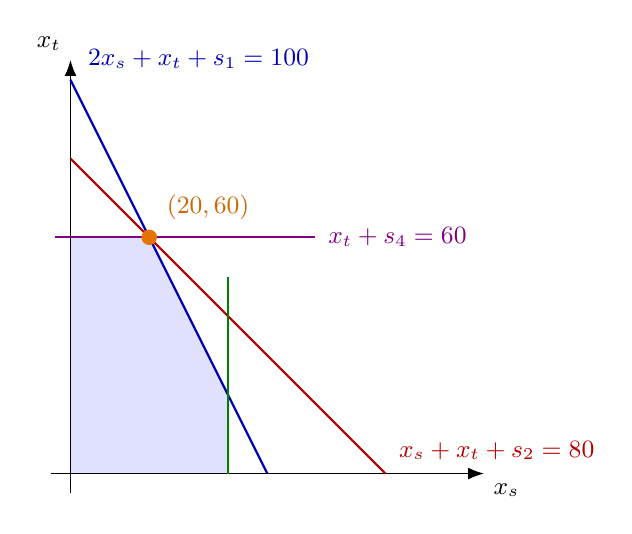
\begin{tikzpicture}[x=0.05cm, y=0.05cm, every node/.style={font=\small}, >={Latex[length=2mm]}]
	\fill[blue!12] (0,0) -- (40,0) -- (40,20) -- (20,60) -- (0,60) -- cycle;
	\draw[->] (-5,0) -- (105,0) node[below right] {$x_s$};
	\draw[->] (0,-5) -- (0,105) node[above left] {$x_t$};
	\draw[blue!70!black, thick] (50,0) -- (0,100);
	\draw[red!70!black, thick] (80,0) -- (0,80);
	\draw[green!50!black, thick] (40,0) -- (40,50);
	\draw[violet, thick] (-4,60) -- (62,60);
	\node[violet, font=\small, anchor=west] at (63,60) {$x_t+s_4=60$};
	\node[blue!70!black, font=\small, anchor=south west] at (2,100.5) {$2x_s+x_t+s_1=100$};
	\node[red!70!black, font=\small, anchor=south west] at (81,1) {$x_s+x_t+s_2=80$};
	\fill[orange!90!black] (20,60) circle (2.8pt);
	\node[orange!80!black, font=\small, anchor=south west] at (22,62) {$(20,60)$};
	\end{tikzpicture}
\end{document}
